% !Mode:: "TeX:UTF-8"
% !TEX program  = xelatex

\documentclass[bwprint]{report}
\setCJKfamilyfont{FZXiaoBiaoSong}{SimHei}

\title{复杂图像的直方图均衡、空间滤波与频域滤波设计与实现}
\stuname{{程泽凯}}
\stuclass{计算机2023-04班}
\supervisor{袁召全 \hspace{1.0em} 老师}
\dateinput{2026年4月}

\begin{document}

\maketitle
\clearpage

% 目录使用Romen页脚
\pagestyle{plain}
\pagenumbering{Roman}
\tableofcontents
\newpage
\pagestyle{plain}

% 正文页脚
\setcounter{page}{1}
\pagenumbering{arabic}

\section{任务背景}
数字图像在采集、传输和显示过程中常会受到光照不足、传感器噪声、纹理干扰以及成像系统模糊等因素影响，导致图像存在对比度偏低、局部细节不明显、噪声点突出或边缘模糊等问题。图像增强的目标不是恢复唯一真实图像，而是在不改变主要内容语义的前提下，使图像中对后续观察、分析和识别更有价值的信息更加明显。

经典图像增强方法可以分为空间域处理和频域处理两类。空间域方法直接作用于像素及其邻域，直观、易实现，适合讲解灰度变换、平滑滤波、顺序统计滤波和锐化算子等基本思想。频域方法则借助傅里叶变换，将图像分解为不同频率分量，从频率角度分析平滑、纹理、边缘和噪声之间的关系。两类方法互为补充：空间域方法便于局部处理，频域方法便于理解全局频率成分的保留与抑制。

\section{任务描述}
本作业要求编程实现复杂图像的直方图均衡及空间滤波，功能包括图像的直方图均衡、图像的线性平滑滤波、顺序统计滤波、使用拉普拉斯算子和一阶微分算子的锐化滤波。同时，还要求实现复杂图像的频域滤波，包括基于傅里叶变换的频域低通滤波和高通滤波。报告需要包含方法基本原理、实现代码、结果分析比较等内容。

本实验采用 Python 作为编程语言，使用 NumPy 完成矩阵运算和傅里叶变换，使用 Pillow 完成图像读写，使用 Matplotlib 生成结果对比图。为了保证实验可复现，实验图像由程序确定性生成，覆盖低对比度、椒盐噪声、边缘块状结构和周期纹理四类典型复杂情况。

\section{技术方案}
\subsection{方案总体架构}
项目结构分为数据生成、算法实现、批量实验、测试验证和模板报告五个部分。核心代码位于 \texttt{src/} 目录，其中 \texttt{histogram\_ops.py} 实现直方图均衡，\texttt{spatial\_filters.py} 实现均值滤波和顺序统计滤波，\texttt{sharpening.py} 实现拉普拉斯锐化和 Sobel 一阶微分锐化，\texttt{frequency\_filters.py} 实现傅里叶频域低通和高通滤波，\texttt{run\_experiments.py} 负责生成图像、调用算法、保存结果和输出统计指标。

\subsection{直方图均衡原理}
直方图反映图像中各灰度级出现的频率。若一幅图像的灰度集中在较窄范围内，则视觉上通常表现为对比度不足。直方图均衡通过构造累计分布函数，将原图灰度重新映射到更宽的灰度范围中。设灰度级为 $r_k$，其概率为 $p(r_k)$，则累计分布变换为
\[
s_k=T(r_k)=\sum_{j=0}^{k}p(r_j).
\]
在 8 位灰度图像中，将 $s_k$ 线性映射到 $[0,255]$ 即可得到新的灰度值。该方法能提升整体对比度，但由于它是全局映射，也可能同时增强局部噪声。

从离散实现角度看，灰度图像共有 $L=256$ 个可能灰度级，设第 $k$ 个灰度级出现次数为 $n_k$，图像总像素数为 $N$，则概率可写为 $p(r_k)=n_k/N$。均衡化本质上是把原图灰度的累计概率作为新灰度的相对位置，即
\[
s_k=\operatorname{round}\left((L-1)\frac{\operatorname{CDF}(r_k)-\operatorname{CDF}_{min}}{N-\operatorname{CDF}_{min}}\right).
\]
其中减去 $\operatorname{CDF}_{min}$ 是为了避免图像中最小有效灰度被映射到非零位置。若图像只有单一灰度值，则分母可能为 0，此时不应强行拉伸，而应直接返回原图。该细节在程序中也进行了判断，保证算法对普通图像和极端图像都稳定。

\subsection{空间滤波原理}
空间滤波直接在像素邻域内完成。线性平滑滤波使用模板对邻域像素进行加权求和，本实验采用 $3\times3$ 均值模板：
\[
g(x,y)=\frac{1}{9}\sum_{i=-1}^{1}\sum_{j=-1}^{1}f(x+i,y+j).
\]
均值滤波可以削弱随机高频变化，但会使边缘和细节变钝。顺序统计滤波不是计算线性加权和，而是将邻域像素排序后取某一统计量。中值滤波取邻域中位数，对孤立的椒盐噪声尤其有效，因为极端黑白噪声在排序后通常不会成为中值。

一般的线性空间滤波可以写成卷积形式：
\[
g(x,y)=\sum_{s=-a}^{a}\sum_{t=-b}^{b}w(s,t)f(x+s,y+t),
\]
其中 $w(s,t)$ 为滤波模板权重。均值滤波的权重全部相等，因此对邻域内所有像素一视同仁，这会降低随机噪声的方差，但也会把真实边缘两侧的灰度混合在一起。顺序统计滤波则属于非线性滤波，不满足卷积叠加关系。以中值滤波为例，它输出排序后的中间值，能有效拒绝最大值和最小值这类异常脉冲。对于图像边界，程序采用边界复制填充，使边界像素仍然可以形成完整邻域，避免输出图像尺寸缩小。

\subsection{锐化滤波原理}
图像锐化的目标是增强灰度变化剧烈的位置。拉普拉斯算子属于二阶微分，本实验使用模板
\[
\begin{bmatrix}
0 & -1 & 0\\
-1 & 4 & -1\\
0 & -1 & 0
\end{bmatrix}.
\]
锐化结果可表示为 $g=f+\alpha\nabla^2 f$。一阶微分采用 Sobel 算子，分别计算水平和垂直方向梯度 $G_x$、$G_y$，再由
\[
G=\sqrt{G_x^2+G_y^2}
\]
得到梯度幅值，并将其按比例叠加回原图。拉普拉斯算子响应强、边缘突出，但对噪声更敏感；Sobel 算子具有方向性，边缘响应较稳定。

从频率含义看，锐化等价于增强高频成分。拉普拉斯算子对灰度曲面的二阶变化敏感，在平坦区域响应接近 0，在边缘或细节突变处响应较大，因此可用于突出轮廓。其缺点是噪声本身也常表现为快速变化，所以二阶微分会放大噪声。Sobel 算子在求一阶差分的同时带有一定加权平滑：中间行或中间列权重为 2，这使它比简单差分更稳定。实际锐化时不能只保留微分响应，否则会丢失原图亮度结构；因此实验采用
\[
g(x,y)=f(x,y)+\alpha R(x,y)
\]
的形式，其中 $R(x,y)$ 为拉普拉斯响应或 Sobel 梯度幅值，$\alpha$ 控制增强强度。

\subsection{频域滤波原理}
二维离散傅里叶变换将图像从空间域变换到频率域。图像整体亮度和缓慢变化主要集中在低频区域，边缘、纹理和噪声通常对应高频区域。频域滤波的一般流程为：对图像做傅里叶变换，移动零频到频谱中心，构造滤波掩模，频谱与掩模相乘，然后进行逆傅里叶变换得到空间域结果。

二维离散傅里叶变换可表示为
\[
F(u,v)=\sum_{x=0}^{M-1}\sum_{y=0}^{N-1}f(x,y)e^{-j2\pi(ux/M+vy/N)}.
\]
其中 $F(0,0)$ 对应图像直流分量，反映平均亮度；靠近中心的频率反映缓慢变化的背景和大尺度结构；远离中心的频率反映细纹理、边缘和噪声。为了便于设计圆形掩模，程序使用 \texttt{fftshift} 将低频移动到频谱中心。滤波后的频谱为
\[
G(u,v)=H(u,v)F(u,v),
\]
再通过逆傅里叶变换得到空间域图像 $g(x,y)$。

本实验采用理想圆形滤波器。低通滤波器定义为
\[
H_L(u,v)=
\begin{cases}
1, & D(u,v)\le D_0,\\
0, & D(u,v)>D_0,
\end{cases}
\]
高通滤波器定义为
\[
H_H(u,v)=
\begin{cases}
0, & D(u,v)<D_0,\\
1, & D(u,v)\ge D_0,
\end{cases}
\]
其中 $D(u,v)$ 为频率点到频谱中心的距离，$D_0$ 为截止半径。

低通滤波保留中心低频区域，适合去除高频噪声和细碎纹理，但图像会变得模糊；高通滤波保留高频区域，适合突出边缘和纹理，但会削弱整体亮度背景。理想滤波器的掩模边界是突变的，理论上可能产生振铃现象。本实验选择理想滤波器主要是为了直观展示“保留低频”和“保留高频”的差异，便于观察傅里叶滤波的基本机制。

\section{实现代码}
本节列出核心实现片段，完整代码保存在作业目录的 \texttt{src/} 下。实现中没有调用 OpenCV 的现成滤波接口，而是使用 NumPy 手写邻域遍历、卷积和频域掩模。

\subsection{直方图均衡}
\begin{lstlisting}[language=Python]
def histogram_equalization(image: np.ndarray) -> np.ndarray:
    if image.ndim != 2:
        raise ValueError("histogram_equalization expects a grayscale image")

    histogram = compute_histogram(image)
    cdf = histogram.cumsum()
    nonzero_cdf = cdf[cdf > 0]
    if nonzero_cdf.size == 0:
        return image.copy()

    cdf_min = nonzero_cdf[0]
    denominator = image.size - cdf_min
    if denominator <= 0:
        return image.copy()

    mapping = np.round((cdf - cdf_min) / denominator * 255.0)
    mapping = np.clip(mapping, 0, 255).astype(np.uint8)
    return mapping[image]
\end{lstlisting}
这段代码首先统计 256 个灰度级的直方图，再对直方图做累加得到累计分布函数 \texttt{cdf}。\texttt{cdf\_min} 用于去掉图像中未出现的低灰度级影响，避免最小有效灰度被映射到非零值。最后构造 \texttt{mapping} 查找表，并通过 \texttt{mapping[image]} 一次性完成所有像素的灰度重映射。这样实现的好处是逻辑与公式一致，并且比逐像素判断更简洁。

\subsection{线性平滑滤波与顺序统计滤波}
\begin{lstlisting}[language=Python]
def linear_smoothing_filter(image: np.ndarray, kernel_size: int = 3) -> np.ndarray:
    _validate_kernel_size(kernel_size)
    padded = _pad_image(image, kernel_size).astype(np.float64)
    result = np.zeros_like(image, dtype=np.float64)

    for row in range(image.shape[0]):
        for col in range(image.shape[1]):
            patch = padded[row : row + kernel_size, col : col + kernel_size]
            result[row, col] = patch.mean()

    return np.clip(np.round(result), 0, 255).astype(np.uint8)

def order_statistic_filter(image: np.ndarray, kernel_size: int = 3, mode: str = "median") -> np.ndarray:
    _validate_kernel_size(kernel_size)
    padded = _pad_image(image, kernel_size)
    result = np.zeros_like(image, dtype=np.float64)

    for row in range(image.shape[0]):
        for col in range(image.shape[1]):
            values = padded[row : row + kernel_size, col : col + kernel_size].reshape(-1)
            if mode == "median":
                result[row, col] = np.median(values)
            elif mode == "min":
                result[row, col] = values.min()
            elif mode == "max":
                result[row, col] = values.max()
            else:
                raise ValueError("mode must be 'median', 'min', or 'max'")

    return np.clip(np.round(result), 0, 255).astype(np.uint8)
\end{lstlisting}
空间滤波代码采用边界复制填充，即 \texttt{mode="edge"}，这样图像边缘位置也能取到完整邻域，输出尺寸与输入保持一致。均值滤波部分对邻域直接求平均，体现线性平滑模板的作用；顺序统计滤波部分先将邻域展开为一维数组，再根据 \texttt{mode} 选择中值、最小值或最大值。本实验主要使用中值模式，它不依赖像素均值，因此对椒盐噪声这类极端值更稳健。

\subsection{拉普拉斯算子与一阶微分锐化}
\begin{lstlisting}[language=Python]
LAPLACIAN_KERNEL = np.array([[0, -1, 0], [-1, 4, -1], [0, -1, 0]], dtype=np.float64)
SOBEL_X_KERNEL = np.array([[-1, 0, 1], [-2, 0, 2], [-1, 0, 1]], dtype=np.float64)
SOBEL_Y_KERNEL = np.array([[-1, -2, -1], [0, 0, 0], [1, 2, 1]], dtype=np.float64)

def laplacian_sharpen(image: np.ndarray, alpha: float = 1.0) -> tuple[np.ndarray, np.ndarray]:
    response = convolve2d(image, LAPLACIAN_KERNEL)
    sharpened = image.astype(np.float64) + alpha * response
    response_view = np.clip(np.abs(np.round(response)), 0, 255).astype(np.uint8)
    result = np.clip(np.round(sharpened), 0, 255).astype(np.uint8)
    return response_view, result

def sobel_sharpen(image: np.ndarray, alpha: float = 0.6) -> tuple[np.ndarray, np.ndarray]:
    gradient = sobel_gradient(image)
    sharpened = image.astype(np.float64) + alpha * gradient
    response_view = np.clip(np.round(gradient), 0, 255).astype(np.uint8)
    result = np.clip(np.round(sharpened), 0, 255).astype(np.uint8)
    return response_view, result
\end{lstlisting}
锐化部分先定义拉普拉斯模板和 Sobel 水平、垂直模板。拉普拉斯锐化通过 \texttt{convolve2d} 计算二阶微分响应，并将响应按系数 \texttt{alpha} 加回原图；Sobel 锐化先计算梯度幅值，再把一阶梯度作为细节增强项叠加回原图。代码中同时返回 \texttt{response\_view} 和 \texttt{result}，前者用于观察算子响应位置，后者是最终增强图像。所有结果都裁剪到 $[0,255]$，保证保存为 8 位灰度图时不会溢出。

\subsection{傅里叶频域低通与高通滤波}
\begin{lstlisting}[language=Python]
def circular_frequency_mask(shape: tuple[int, int], cutoff: float, mode: str) -> np.ndarray:
    rows, cols = shape
    center_row = rows // 2
    center_col = cols // 2
    y_grid, x_grid = np.ogrid[:rows, :cols]
    distance = np.sqrt((y_grid - center_row) ** 2 + (x_grid - center_col) ** 2)
    if mode == "low":
        return (distance <= cutoff).astype(np.float64)
    return (distance >= cutoff).astype(np.float64)

def apply_frequency_filter(image: np.ndarray, cutoff: float, mode: str) -> tuple[np.ndarray, np.ndarray, np.ndarray]:
    frequency = np.fft.fftshift(np.fft.fft2(image.astype(np.float64)))
    mask = circular_frequency_mask(image.shape, cutoff=cutoff, mode=mode)
    filtered_frequency = frequency * mask
    reconstructed = np.fft.ifft2(np.fft.ifftshift(filtered_frequency))
    if mode == "low":
        result = np.clip(np.round(np.real(reconstructed)), 0, 255).astype(np.uint8)
    else:
        high_component = np.abs(np.real(reconstructed))
        high_component = high_component / high_component.max() * 255.0
        result = np.clip(np.round(high_component), 0, 255).astype(np.uint8)
    return mask, np.log1p(np.abs(filtered_frequency)), result
\end{lstlisting}
频域滤波代码中，\texttt{circular\_frequency\_mask} 根据频谱坐标到中心点的距离构造圆形掩模。低通模式保留中心低频区域，高通模式保留远离中心的高频区域。\texttt{apply\_frequency\_filter} 先做二维傅里叶变换并用 \texttt{fftshift} 将低频移动到中心，再用掩模逐点相乘，最后通过逆变换回到空间域。高通结果只保留变化分量，直接显示会偏暗，因此代码对高频幅值做归一化，便于在报告图中观察边缘和纹理。

\section{实验}
\subsection{数据集与实验设置}
实验自建四幅 $512\times512$ 灰度图像。第一幅为低对比度场景，主要用于验证直方图均衡；第二幅为带椒盐噪声的纹理图像，主要用于比较均值滤波与中值滤波；第三幅为边缘块状图像，用于观察锐化算子的边缘增强效果；第四幅为周期纹理图像，用于展示频域低通和高通滤波对不同频率成分的选择性。

实验命令如下：
\begin{lstlisting}[language=bash]
python src/run_experiments.py
pytest -q
\end{lstlisting}
其中空间滤波模板大小为 $3\times3$，频域滤波截止半径为 28 像素。测试结果为 9 个用例全部通过，说明各核心函数在输出尺寸、数据类型、数值范围和基本行为上符合预期。

\subsection{直方图均衡结果}
\begin{figure}[H]
    \centering
    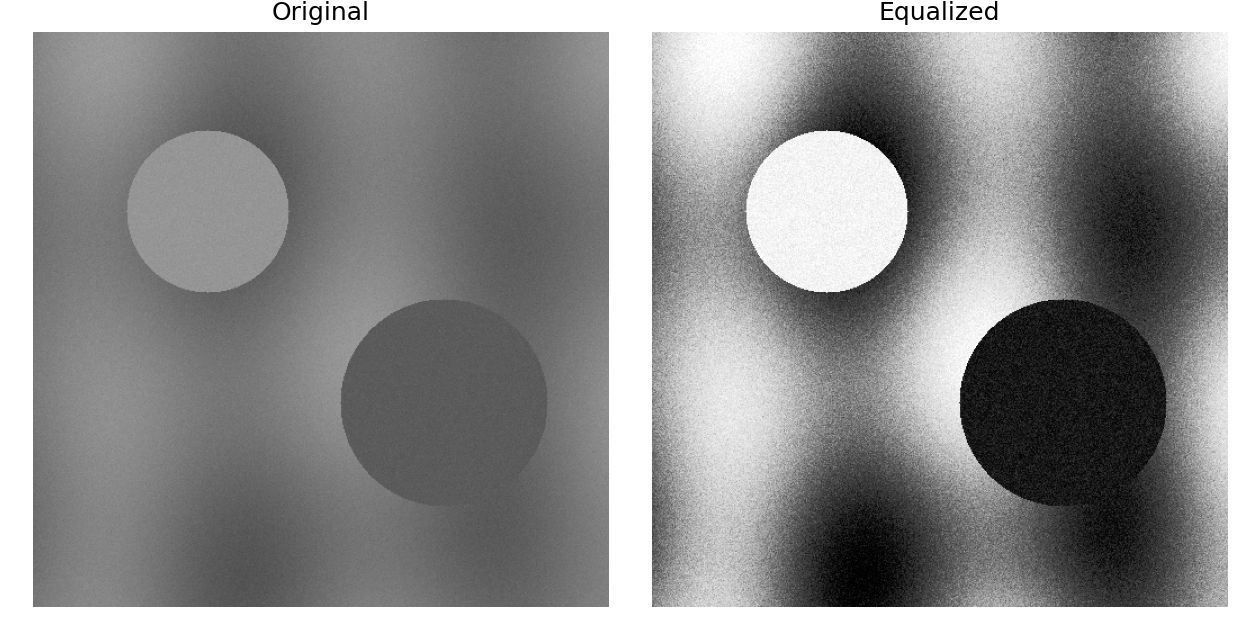
\includegraphics[width=0.92\textwidth]{figures/low_contrast_scene_histogram_compare.png}
    \caption{低对比度图像直方图均衡前后对比}
    \label{fig:hist}
\end{figure}

如图 \ref{fig:hist} 所示，原图灰度集中在较窄范围，均衡后图像整体层次更清晰，暗部和亮部差异更明显。统计结果显示，低对比度图像的灰度标准差由 18.07 提升到 73.48，说明灰度动态范围明显扩展。该结果验证了全局直方图均衡提升整体对比度的作用。

\subsection{空间滤波结果}
\begin{figure}[H]
    \centering
    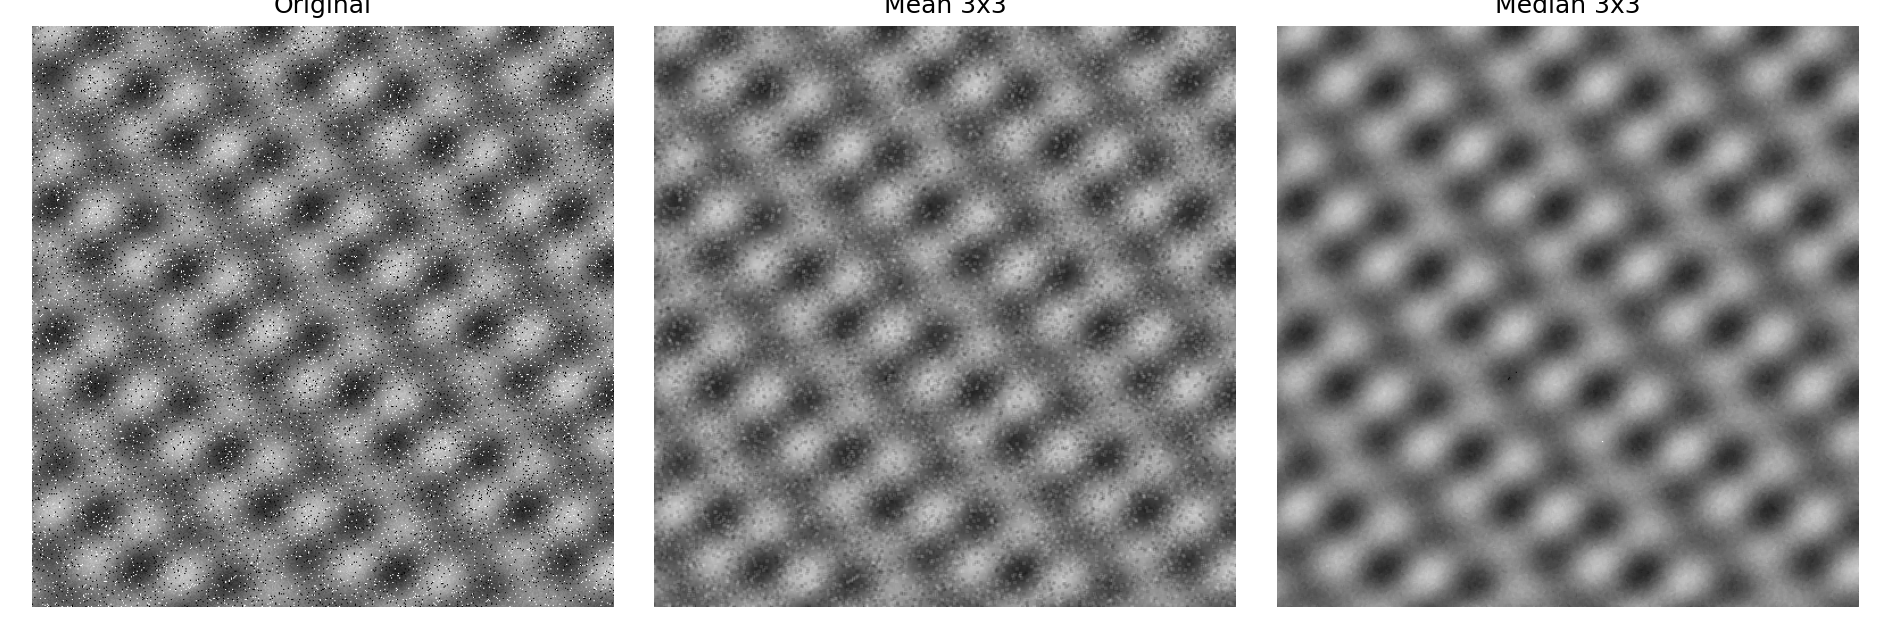
\includegraphics[width=0.95\textwidth]{figures/salt_pepper_texture_spatial_compare.png}
    \caption{椒盐噪声图像的均值滤波与中值滤波对比}
    \label{fig:spatial}
\end{figure}

如图 \ref{fig:spatial} 所示，均值滤波能平滑整体纹理，但会将黑白脉冲点的影响扩散到邻域，使局部细节变软；中值滤波对孤立椒盐噪声的抑制更直接，保留结构也更自然。该图像中原始极值脉冲像素为 18286 个，均值滤波后极值像素为 0 个，中值滤波后仅剩 5 个，说明中值滤波对该类噪声具有更强针对性。

\subsection{锐化滤波结果}
\begin{figure}[H]
    \centering
    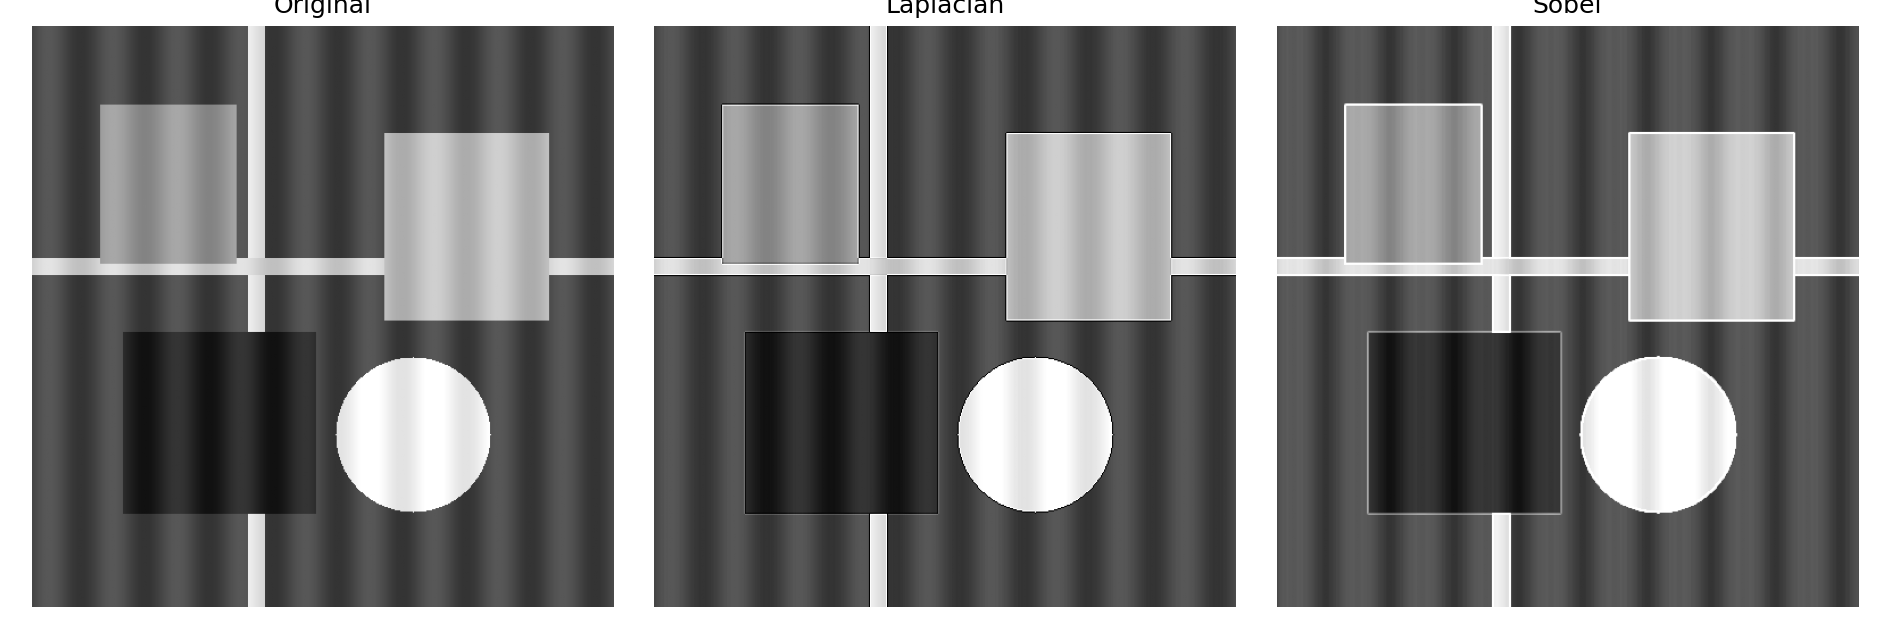
\includegraphics[width=0.95\textwidth]{figures/edge_blocks_sharpen_compare.png}
    \caption{边缘块状图像的拉普拉斯锐化与 Sobel 锐化对比}
    \label{fig:sharp}
\end{figure}

如图 \ref{fig:sharp} 所示，拉普拉斯算子和 Sobel 算子都能增强边缘。边缘块状图像的平均梯度由 21.65 提升到约 32.8，说明边界变化被强化。拉普拉斯结果对灰度突变响应更强，边缘更硬；Sobel 结果方向性更明显，整体增强更平稳。若原图噪声较强，拉普拉斯算子更容易同步放大噪声，因此实际应用中常需要先做适度平滑。

\subsection{频域滤波结果}
\begin{figure}[H]
    \centering
    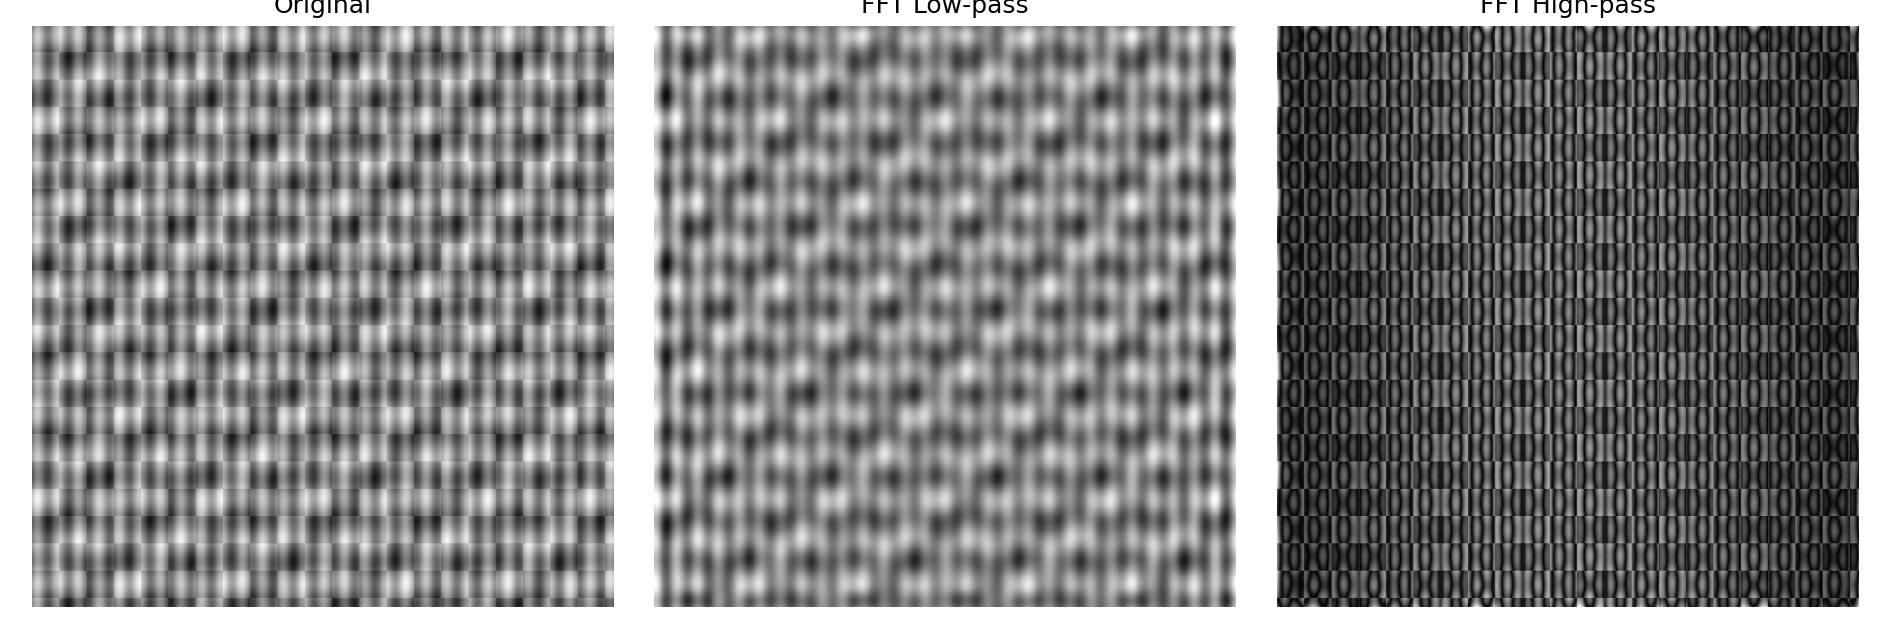
\includegraphics[width=0.95\textwidth]{figures/frequency_pattern_frequency_compare.png}
    \caption{周期纹理图像的傅里叶低通与高通滤波对比}
    \label{fig:freq}
\end{figure}

\begin{figure}[H]
    \centering
    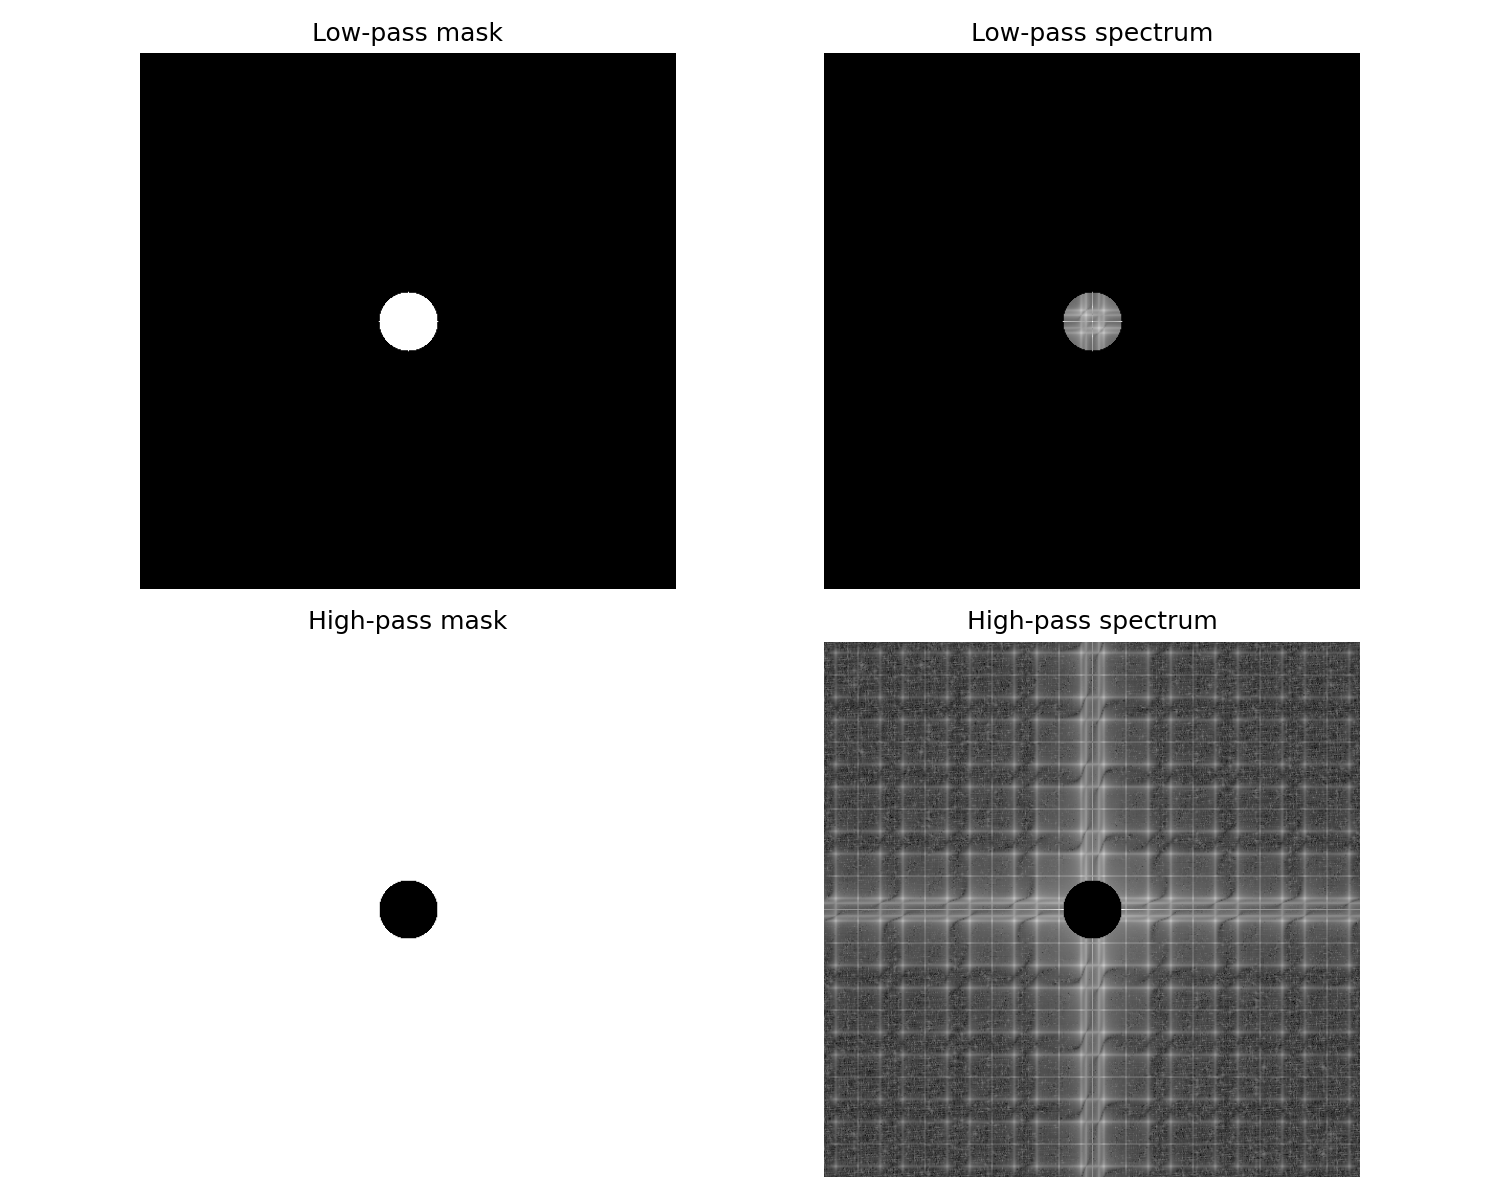
\includegraphics[width=0.78\textwidth]{figures/frequency_pattern_frequency_detail.png}
    \caption{频域低通与高通滤波的掩模和滤波后频谱}
    \label{fig:freq_detail}
\end{figure}

图 \ref{fig:freq} 和图 \ref{fig:freq_detail} 展示了频域滤波的效果。低通滤波保留频谱中心区域，使周期纹理和边缘细节被削弱，图像变得平滑；高通滤波抑制低频背景，保留快速变化成分，使条纹和边缘更加突出。周期纹理图像的高频能量比例由 0.0446 降到 0.0226，说明低通滤波确实削弱了高频成分。

\subsection{定量结果汇总}
\begin{table}[H]
    \centering
    \caption{不同图像上的统计指标对比}
    \resizebox{\textwidth}{!}{
    \begin{tabular}{lrrrrrrrr}
        \toprule
        图像 & 原始STD & 均衡STD & 原始梯度 & 拉普拉斯梯度 & Sobel梯度 & 原始高频比 & 低通高频比 & 高通高频比 \\
        \midrule
        edge\_blocks & 60.90 & 73.75 & 21.65 & 32.80 & 33.04 & 0.0134 & 0.0002 & 0.2920 \\
        frequency\_pattern & 43.20 & 73.68 & 91.38 & 129.83 & 133.37 & 0.0446 & 0.0226 & 0.2233 \\
        low\_contrast\_scene & 18.07 & 73.48 & 16.48 & 61.50 & 30.63 & 0.0014 & 0.0000 & 0.3312 \\
        salt\_pepper\_texture & 46.34 & 76.26 & 129.30 & 188.40 & 237.27 & 0.0763 & 0.0000 & 0.7930 \\
        \bottomrule
    \end{tabular}}
    \label{tab:metrics}
\end{table}

表 \ref{tab:metrics} 从数值上支持了前述观察。直方图均衡普遍提高灰度标准差，其中低对比度场景提升最明显；锐化后平均梯度增大，说明边缘和纹理响应增强；低通滤波后的高频比例明显下降，高通滤波输出中的高频占比更高，说明频域掩模按预期保留或抑制了相应频率成分。

\section{结果分析比较}
从实验现象看，直方图均衡适合处理整体对比度不足的图像，其优点是实现简单、效果直观，但缺点是缺少局部自适应能力，可能放大噪声。均值滤波适合一般随机噪声抑制，但边缘保持能力较弱；中值滤波属于非线性顺序统计方法，对椒盐噪声更有效，且比均值滤波更能保留突变边界。拉普拉斯锐化强调二阶变化，边缘增强明显，但对噪声敏感；Sobel 一阶微分通过方向梯度描述边缘，响应更平稳，适合作为边缘检测和温和锐化的基础。

频域低通和高通滤波从另一个角度解释了平滑与锐化的本质。平滑可以看作削弱高频分量，锐化可以看作突出高频分量。与空间域模板相比，频域方法能更直观地观察不同频率成分的保留情况，但理想滤波器边界突变明显，在真实图像中可能引入振铃现象。若进一步改进，可采用高斯低通、高斯高通或巴特沃斯滤波器，以获得更平滑的频率过渡。

\section{总结}
本作业在指定课程模板副本中完成了复杂图像增强实验报告，并编程实现了题目要求的全部功能：图像直方图均衡、线性平滑滤波、顺序统计滤波、拉普拉斯锐化、一阶微分锐化、傅里叶频域低通滤波和傅里叶频域高通滤波。实验结果表明，不同方法对应不同图像问题：直方图均衡主要改善灰度分布，空间平滑主要抑制噪声，中值滤波适合椒盐噪声，锐化滤波增强边缘细节，频域滤波则可以从频率成分角度实现平滑和增强。

通过本次实验，可以更清楚地理解空间域和频域图像处理方法之间的联系：图像中的边缘、纹理和噪声通常表现为高频信息，而整体亮度和大尺度结构主要表现为低频信息。实际应用中需要结合图像退化类型选择方法，必要时将平滑、均衡和锐化组合使用，才能在噪声抑制、细节保持和视觉增强之间取得较好的平衡。

\end{document}
